\documentclass[UTF8,a4paper,zihao=-4]{ctexart}
\usepackage{amsmath,amssymb}
\usepackage{booktabs,longtable,array}
\usepackage{graphicx}
\usepackage[numbers,square]{natbib}
\usepackage[margin=2.2cm]{geometry}
\usepackage{fancyhdr}
\usepackage[colorlinks=true,linkcolor=black,urlcolor=blue]{hyperref}

\ctexset{
  section={format=\centering\heiti\zihao{4},name={},number={},aftername=},
  subsection={format=\heiti\zihao{-4},name={},number={\thesection.\arabic{subsection}},aftername=\quad},
  subsubsection={format=\heiti\zihao{-4},name={},number={\thesubsection.\arabic{subsubsection}},aftername=\quad}
}
\setlength{\parindent}{2em}
\setlength{\parskip}{0pt}
\linespread{1.0}
\pagestyle{fancy}
\fancyhf{}
\fancyfoot[C]{\thepage}
\renewcommand{\headrulewidth}{0pt}
\renewcommand{\footrulewidth}{0pt}
\hypersetup{
  pdftitle={山区洪涝灾害下无人机运输与通信协同优化},
  pdfauthor={},
  pdfsubject={D题数学建模论文},
  pdfkeywords={无人机运输；多架次调度；通信中继；资源分区}
}

\newcommand{\papertitle}{山区洪涝灾害下无人机运输与通信协同优化}

\begin{document}

% 独立封面承载参赛身份信息；正文、摘要及PDF元数据保持匿名。
\thispagestyle{empty}
\begin{center}
  {\zihao{3}\heiti 中国研究生创新实践系列大赛\par}
  \vspace{0.5em}
  {\zihao{3}\heiti “华为杯”第二十三届中国研究生数学建模竞赛\par}
  \vspace{4em}
  {\zihao{2}\heiti 竞赛论文\par}
  \vspace{3em}
  {\zihao{3}\heiti \papertitle\par}
\end{center}
\vfill
\begin{center}
  \zihao{-3}
  \renewcommand{\arraystretch}{1.8}
  \begin{tabular}{rl}
    队伍编号：& 26106980342 \\
    队伍名称：& 哦 \\
    单位名称：& 西安交通大学 \\
    队员：& 丁金、祁迹昂、孙家兴
  \end{tabular}
\end{center}
\vfill
\clearpage

% 竞赛要求从摘要页开始连续编页码，摘要页与正文均不出现身份信息。
\pagenumbering{arabic}
\setcounter{page}{1}
\thispagestyle{fancy}
\begin{center}
  {\zihao{3}\heiti \papertitle\par}
  \vspace{1em}
  {\zihao{4}\heiti 摘要\par}
\end{center}
\vspace{0.5em}
\noindent\zihao{-4}\songti
针对山区洪涝灾害下应急物资运输、有限机队与电池周转以及通信中继保障问题，本文建立由单点运输能力评估、多架次联合调度、通信保障优化和灾后任务分区构成的递进模型。问题一依据地形剖面、载荷修正航程和爬升能耗计算安全载荷，并以动态规划精确组批；问题二构造跨服务区候选架次池，将货箱覆盖、机型选择、访问顺序、无人机占用和电池充电周转联合求解；问题三在运输调度基础上联合优化中继驻守与服务窗口，并校验链路可用性；问题四冻结问题三任务，按运输架次继承关系划分服务区，比较两组与三组方案的峰值资源和工作量均衡。

问题一得到18个运输架次的精确组批方案，达到由三个超载服务区给出的架次数下界；默认20\%返航安全余量下总能耗为59.2403~kWh。问题二在80箱全部按期交付、硬时限及期望时刻迟到均为零的条件下，得到22个架次，最晚返场时间5830.8212~s，总能耗67.4469~kWh。问题三在该运输基线上重新调整两个医疗箱的批次归属及中继点，得到22个运输架次、3个中继架次，联合完成时间6926.1512~s，总能耗68.5635~kWh；独立离散采样未发现通信中断，但不将采样结果表述为连续时间严格证明。问题四穷举11个不可拆分单元的两组与三组划分，均得到工作量变异系数不超过0.10的方案；在完整中继任务窗口按组独立复制的保守假设下，两组方案的工作量变异系数为0.0269，库存缺口为6个资源单位，优于三组方案的0.0856和10个资源单位。

本文的主要特点是利用货箱类型聚合压缩组合搜索空间，并将多站运输、有限电池充电和中继实体周转纳入统一的事件驱动调度；对问题四则明确区分题面约束与保守资源核算假设，并对冻结输入下的候选分区作穷举比较。所得调度与分区均为所述模型和假设下的可行或最优结果，不据此宣称问题二至四的全局最优。

\vspace{0.6em}
\noindent{\heiti 关键词：}山区洪涝；无人机运输；多架次调度；电池周转；通信中继；任务分区
\clearpage

\section{问题一：单点往返运输能力与货箱组批}

\subsection{问题分析}

问题一不考虑实体无人机数量及共享电池周转，每个架次均采用
$O01\rightarrow S_i\rightarrow O01$ 的直接往返形式，且一个架次只能服务一个服务区。
因此，该问题可分为两个相互衔接的子问题：首先利用地形、航程和能量约束反解三种机型到各服务区的最大安全载荷；随后将同一服务区内不可拆分的货箱划分为若干批次，并联合选择机型，使架次数、运输能耗和累计作业时间尽可能小。

附件中的80个货箱只有4种质量--体积组合。利用这一离散结构，可以按箱型计数而非逐箱枚举，从而在较小状态空间内进行精确动态规划。考虑到灾后早期的组织负担和飞行风险，本文采用字典序多目标：首先最小化架次数，在此基础上最小化总能耗，最后最小化累计作业时间。

\subsection{航段几何、时间与能耗模型}

设机型集合为 $G=\{A,B,C\}$，服务区集合为 $S=\{S_1,\ldots,S_{15}\}$。
对任意节点 $i,j$，以两节点经纬度之间的测地距离作为水平巡航距离 $d_{ij}$。沿直线航段查询30~m DEM，记经过像元的最高高程为 $H_{ij}^{\max}$，则计划巡航海拔为
\begin{equation}
H_{ij}^{\mathrm{cruise}}=H_{ij}^{\max}+50.
\end{equation}
调度中心作业海拔取附件给定地面海拔，服务区作业海拔取地面海拔加30~m。由此得到航段爬升高度 $h_{ij}^{+}$ 和下降高度 $h_{ij}^{-}$。

机型 $g$ 携带载荷 $q$ 时的等效航程严格按题面给出的 $3/2$ 次幂关系计算。旋翼动量理论中的诱导功率随推力呈 $3/2$ 次幂变化，相关无人机配送能耗模型也讨论了载荷与能耗的联系；本文仍以题面公式为计算口径，不直接移用文献参数或数值结论\cite{zhang2021}：
\begin{equation}
L_g(q)=L_{g0}-\left(L_{g0}-L_{gF}\right)
\left(\frac{q}{Q_g}\right)^{3/2},\qquad 0\le q\le Q_g,
\end{equation}
其中，$L_{g0}$、$L_{gF}$ 和 $Q_g$ 分别为空载标准航程、满载标准航程和最大载货质量。
将单组电池可用能量 $E_g^{\mathrm{use}}$ 除以等效航程，得到单位水平距离能耗。航段总能耗为
\begin{equation}
E_{g,ij}(q)=\frac{E_g^{\mathrm{use}}}{L_g(q)}d_{ij}
+\frac{(m_g+q)g_0h_{ij}^{+}}{3.6\times10^6\eta_g},
\end{equation}
其中 $m_g$ 为空机质量，$g_0=9.80665~\mathrm{m/s^2}$，$\eta_g$ 为爬升能耗效率。按照题面规定，下降过程不单独计算附加能耗。

单点投送后货物已全部卸载，故返程有效载荷为0。载质量为 $q$ 的往返架次能耗为
\begin{equation}
E_{g,i}^{\mathrm{rt}}(q)=E_{g,O01,i}(q)+E_{g,i,O01}(0).
\end{equation}
若本架次装载 $n$ 个货箱，其完整作业时间为
\begin{equation}
T_{g,i}(n)=T_g^{\mathrm{prep}}+T_g^{\mathrm{load}}n
+\sum_{(u,v)\in\{(O01,i),(i,O01)\}}
\left(\frac{h_{uv}^{+}}{v_g^{\uparrow}}+\frac{d_{uv}}{v_g^c}+\frac{h_{uv}^{-}}{v_g^{\downarrow}}\right)
+T_g^{\mathrm{handoff}}+T_g^{\mathrm{perbox}}n.
\end{equation}
该式同时计入固定准备、逐箱装载、往返飞行、基础交接和逐箱交接时间。由于问题一明确不考虑实体无人机调度，本文将所有架次完整作业时间之和作为“累计作业时间”，不将其解释为多机并行条件下的完工时间。

\subsection{最大安全载荷反解}

设机型 $g$ 的返航安全余量为 $\rho_g$。最大安全载荷 $q_{g,i}^{\max}$ 满足
\begin{equation}
q_{g,i}^{\max}=\max\left\{q:\ 0\le q\le Q_g,
\ E_{g,i}^{\mathrm{rt}}(q)\le(1-\rho_g)E_g^{\mathrm{use}}\right\}.
\end{equation}
由于 $L_g(q)$ 随载荷单调减小，往返能耗随载荷单调增加，故采用二分法求解该一维边界。取附件默认安全余量 $\rho_g=20\%$，结果见表~\ref{tab:q1-payload}。

\begin{table}[htbp]
\centering
\caption{20\%返航安全余量下各机型最大安全载荷（kg）}
\label{tab:q1-payload}
\small
\begin{tabular}{cccccccc}
\toprule
服务区 & A型 & B型 & C型 & 服务区 & A型 & B型 & C型\\
\midrule
S001 & 25.000 & 30.000 & 80.000 & S009 & 25.000 & 30.000 & 80.000\\
S002 & 25.000 & 30.000 & 68.554 & S010 & 25.000 & 30.000 & 80.000\\
S003 & 25.000 & 30.000 & 68.235 & S011 & 25.000 & 30.000 & 80.000\\
S004 & 25.000 & 30.000 & 63.259 & S012 & 25.000 & 30.000 & 68.015\\
S005 & 25.000 & 30.000 & 80.000 & S013 & 25.000 & 30.000 & 80.000\\
S006 & 25.000 & 30.000 & 80.000 & S014 & 25.000 & 30.000 & 80.000\\
S007 & 25.000 & 30.000 & 80.000 & S015 & 25.000 & 30.000 & 80.000\\
S008 & 25.000 & 28.632 & 58.436 & & & &\\
\bottomrule
\end{tabular}
\end{table}

结果表明，A型除受自身25~kg载荷上限约束外，在全部服务区均可满载；B型仅在S008受能量约束而不能满载；C型在S002、S003、S004、S008和S012受长航程或较大爬升高度影响，最大安全载荷低于80~kg。各服务区载荷边界及机型额定载荷对照见图~\ref{fig:q1-payload}。
\begin{figure}[htbp]
\centering
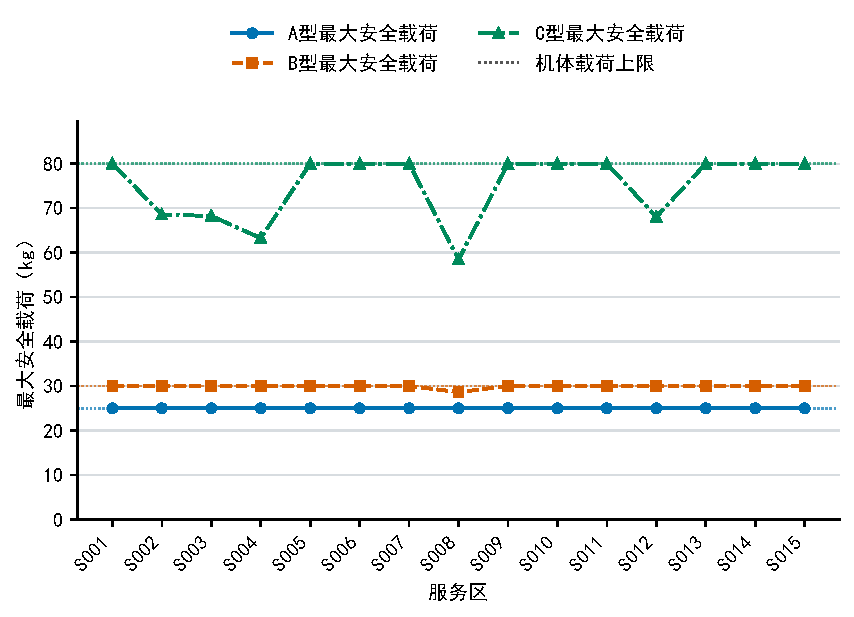
\includegraphics[width=0.96\textwidth]{figures/q1_payload_by_service.pdf}
\caption{20\%返航安全余量下各服务区的机型最大安全载荷}
\label{fig:q1-payload}
\end{figure}

\subsection{跨机型货箱组批模型}

将医疗物资、饮用水、应急食品和生活卫生用品依次记为4种箱型。对服务区 $i$，用向量 $\boldsymbol{b}_i$ 表示各箱型需求数量。枚举机型 $g$ 下所有满足质量、体积和能量限制的装载组合，构成可行选项集合 $\mathcal{F}_i$。对选项 $r\in\mathcal{F}_i$，记其箱型计数向量为 $\boldsymbol{a}_r$，能耗和作业时间分别为 $e_r,t_r$，决策变量 $x_r$ 表示该选项使用的架次数。模型为
\begin{align}
\operatorname{lexmin}\quad &
\left(\sum_{r\in\mathcal{F}_i}x_r,
\sum_{r\in\mathcal{F}_i}e_rx_r,
\sum_{r\in\mathcal{F}_i}t_rx_r\right),\\
\text{s.t.}\quad &
\sum_{r\in\mathcal{F}_i}\boldsymbol{a}_rx_r=\boldsymbol{b}_i,\\
&x_r\in\mathbb{Z}_{\ge0}.
\end{align}
等式约束保证每个货箱恰好分配一次；可行选项的生成过程已经内嵌载质量、装载体积和返航安全余量约束。

求解时以“尚未分配的4类货箱数量”为动态规划状态。对每个状态枚举一个可行架次，转移到扣除对应货箱后的新状态，并依次比较架次数、累计能耗和累计时间。全题单服务区最大状态数为 $(2+1)(8+1)(3+1)(2+1)=324$，三种机型对应的候选装载上界不足 $3\times323=969$，可对全部状态和选项进行穷尽搜索。所得解是上述字典序目标下的精确最优解，不依赖随机初值，也不存在启发式算法的收敛误差。

\subsection{组批结果与多目标权衡}

各服务区联合最优结果见表~\ref{tab:q1-plan-summary}，逐箱货箱编号及每架次质量、体积、能耗、时间和返航SOC见结果附件。

\begin{table}[htbp]
\centering
\caption{各服务区联合最优组批结果}
\label{tab:q1-plan-summary}
\small
\begin{tabular}{ccrrr}
\toprule
服务区 & 机型组合 & 架次数 & 能耗/kWh & 时间/s\\
\midrule
S001 & C+C & 2 & 5.9309 & 3188.9\\
S002 & C+B & 2 & 8.4612 & 3864.9\\
S003 & C+B & 2 & 8.5424 & 4450.1\\
S004 & C & 1 & 6.1769 & 2305.2\\
S005 & C & 1 & 4.2387 & 1880.0\\
S006 & C & 1 & 2.5939 & 1560.9\\
S007 & C & 1 & 3.4104 & 1907.5\\
S008 & C & 1 & 5.8575 & 2203.8\\
S009 & B & 1 & 2.1024 & 1560.8\\
S010 & B & 1 & 1.8210 & 1554.6\\
S011 & B & 1 & 1.0771 & 1189.6\\
S012 & B & 1 & 2.7552 & 1923.8\\
S013 & B & 1 & 1.8245 & 1510.4\\
S014 & B & 1 & 2.1372 & 1868.6\\
S015 & B & 1 & 2.3108 & 1829.6\\
\midrule
合计 & B型9+C型9 & 18 & 59.2403 & 32798.5\\
\bottomrule
\end{tabular}
\end{table}

18架次不仅是算法得到的结果，也可由下界证明。每个服务区至少需要1架次；S001、S002和S003的需求总质量分别为154、81和81~kg，均超过单架最大载荷80~kg，故三者各至少需要2架次。因此总架次数下界为
\begin{equation}
15+3=18,
\end{equation}
本文方案达到该下界，故架次数全局最优。

为说明三个目标之间的权衡，分别限制全程只使用一种机型，并与跨机型联合方案比较，结果见表~\ref{tab:q1-tradeoff}。

\begin{table}[htbp]
\centering
\caption{不同机型策略的指标比较}
\label{tab:q1-tradeoff}
\begin{tabular}{lrrr}
\toprule
策略 & 架次数 & 总能耗/kWh & 累计作业时间/s\\
\midrule
仅A型 & 52 & 112.383 & 89415.8\\
仅B型 & 35 & 68.478 & 55708.7\\
仅C型 & 18 & 74.058 & 33861.2\\
跨机型联合优化 & 18 & 59.2403 & 32798.5\\
\bottomrule
\end{tabular}
\end{table}

仅使用C型已能达到最少架次数，但在小批量服务区存在“大机小载”现象。联合方案保持18架次不变，同时用B型承担S009--S015以及S002、S003中的小批量，使能耗较仅C型下降约20.0\%，累计作业时间下降约3.1\%。这说明“最少架次数”并不自动对应“最低能耗”，异构机型组合能够改善次级目标。

\subsection{安全余量灵敏度分析}

以附件默认值20\%为中心，为同时覆盖宽松情景与方案失效边界，将返航安全余量 $\rho$ 从0逐步提高到40\%，每个取值下重新生成可行装载组合并执行跨机型联合优化。

\begin{table}[htbp]
\centering
\caption{返航安全余量对全局组批方案的影响}
\label{tab:q1-sensitivity}
\small
\begin{tabular}{crrrccc}
\toprule
$\rho$ & 架次数 & 总能耗/kWh & 时间/s & A型 & B型 & C型\\
\midrule
0\%--20\% & 18 & 59.2403 & 32798.5 & 0 & 9 & 9\\
25\% & 19 & 61.1897 & 34592.3 & 0 & 10 & 9\\
30\% & 20 & 67.3577 & 36616.8 & 0 & 9 & 11\\
35\% & 25 & 78.1856 & 45550.8 & 0 & 14 & 11\\
40\% & \multicolumn{6}{c}{不可行}\\
\bottomrule
\end{tabular}
\end{table}

在0--20\%范围内，18架次方案及机型结构保持不变，说明默认20\%余量下结论稳定。当余量升至25\%时，部分长航程服务区的单架安全载荷跨过组批临界值，架次数增至19；30\%和35\%时进一步增至20和25。余量达到40\%后，S004、S008等长航程服务区出现至少一种较重货箱无法由任何机型安全运输的情况，问题转为不可行。因此，20\%是兼顾安全性与运输效率的稳定取值，而25\%是当前方案架次数发生变化的首个临界点。全局架次、能耗和累计作业时间的变化趋势见图~\ref{fig:q1-sensitivity}；40\%处因不存在可行装载组合而停止绘制指标值。
\begin{figure}[htbp]
\centering
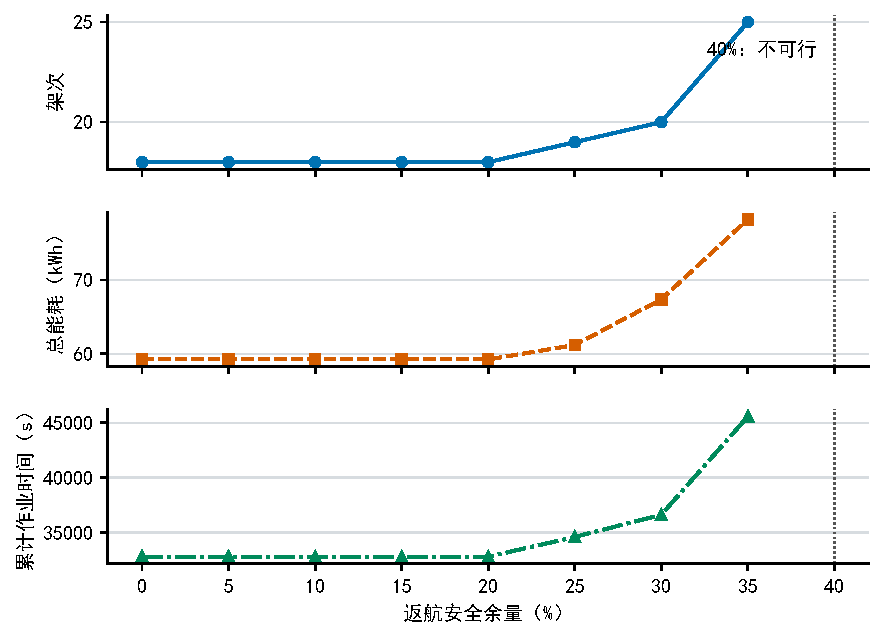
\includegraphics[width=0.96\textwidth]{figures/q1_global_reserve_sensitivity.pdf}
\caption{返航安全余量对全局组批方案指标的影响}
\label{fig:q1-sensitivity}
\end{figure}

\subsection{模型检验与误差讨论}

本文从以下方面进行独立复核：其一，检查 $L_g(0)=L_{g0}$、$L_g(Q_g)=L_{gF}$ 以及载荷增加时能耗单调增加；其二，重新读取逐箱结果，验证80个货箱恰好出现一次，总质量758.0~kg、总体积2.011~m$^3$，并逐架次复算质量、体积、能量、时间和SOC；其三，以18架次解析下界验证动态规划的最优性。上述检查均通过。程序在Python~3.13环境下运行，主要使用NumPy~2.2.5、SciPy~1.15.3和openpyxl~3.1.5；求解入口与独立检查入口分别为 \texttt{q1\_sensitivity.py} 和 \texttt{q1\_validate.py}。

误差主要来自三个方面：DEM为空间分辨率约30~m的栅格数据，航段最高高程受像元采样影响；附件节点海拔与DEM采样值存在不超过10.6~m的偏差，本文按题意以附件海拔作为作业高度、DEM仅用于沿线净空；等效航程模型把实际复杂飞行过程折算为确定性单位距离能耗，未显式考虑风速和电池老化。为评估空间离散误差，将沿线采样密度由每像元跨度约1点提高到8点，个别航段最高高程最多增加10.14~m，总能耗由59.2232增至59.2403~kWh（约0.03\%），累计时间由32755.1增至32798.5~s（约0.13\%），18架次及B型9架次、C型9架次的结构保持不变。由于题目未提供风场与电池老化数据，这些因素不纳入主模型，其影响通过返航安全余量吸收。安全余量灵敏度结果表明，在0--20\%范围内最优架次数和机型结构均不变，故上述误差不足以改变问题一的核心结论。

\section{问题二：异构无人机多点多架次调度}

\subsection{问题分析与总体框架}

问题二要求同时确定货箱组批、访问顺序、运输机型、实体无人机、共享电池和开始时刻。与问题一相比，新增难点不是单一航段的物理计算，而是路线、实体机与电池充电时间线之间的耦合。多架次复用和配送完成时间的联合优化是无人机配送研究中的相关建模方向\cite{dorling2017}；本文的约束、参数与数值均依据题面和本题数据重新建立。本文采用事件驱动方法，只记录架次开始、逐站交付、返回和充电完成四类事件，避免按秒离散整个任务周期。

初步方案以压缩架次为主要目标，将大量后续任务集中到两架C型无人机，虽可降至19架次，却形成串行瓶颈，导致8箱普通物资迟到，最晚返场达到13806.3~s。根据该诊断，最终模型将目标优先级改为：硬时限可行、普通物资零迟到、最晚返场时间最小、总能耗较低，最后才考虑架次数。

\subsection{多点架次的时间与能耗}

设架次 $r$ 的访问顺序为
\[
O01\rightarrow v_{r1}\rightarrow \cdots\rightarrow v_{rm_r}\rightarrow O01,
\]
初始装载货箱集合为 $B_r$。进入第 $k$ 个航段前的剩余载荷为
\[
q_{rk}=\sum_{b\in B_r:\,b\text{ 尚未交付}}m_b.
\]
每到一个服务区完成交付后扣除该站货箱质量，再从服务区作业高度重新爬升。架次能耗为
\[
E_r=\sum_{k=0}^{m_r}E_{g_r}\!\left(q_{rk},v_{rk},v_{r,k+1}\right),
\qquad E_r\leq (1-\rho_{g_r})E^{\rm use}_{g_r},
\]
其中最后一个返航航段载荷为0，单航段能耗沿用问题一的等效航程和爬升势能模型；载荷航程严格采用题目给定的 $3/2$ 次幂修正。

设架次开始时刻为 $s_r$，货箱 $b$ 在所属服务区交接结束时刻记为 $t_b$。医疗物资满足 $t_b\leq d_b^{\rm exp}$，首批保障货箱满足 $t_b\leq d_b^{\rm first}$。其余货箱的加权迟到量为
\[
D=\sum_{b\in B^{\rm soft}}w_b\max\{0,t_b-d_b^{\rm exp}\}.
\]

\subsection{实体无人机与共享电池调度}

同一实体无人机的任意两个架次区间不得重叠。电池从架次开始至返航均视为被占用，返航荷电状态为
\[
SOC_r=1-\frac{E_r}{E_{g_r}^{\rm use}}.
\]
返航后立即按附件的两阶段模型充电。若电池 $p$ 连续执行架次 $r$ 和 $r'$，则
\[
s_{r'}\geq C_r+t_{\rm chg}(SOC_r),
\]
其中 $C_r$ 为架次返回时刻。不同电池可并行充电，A、B、C型电池不可跨机型使用。调度时枚举同机型实体机与电池的组合，并取两者最早可用时刻的较大值作为候选开始时刻。

\subsection{候选组批池与资源约束排程}

早期方法固定首波机型后作局部交换，得到22架次、6977.52~s的可行方案，但7个C型架次总工作量约13537~s，两架C型机的纯工作量下界已超过6768~s，无法仅通过调整开始时刻达到6000~s。因此本轮保持22架次和全部货箱零迟到，开放跨区组批与首波机型选择。

将服务区、质量、体积及有效截止时刻完全相同的货箱合并为53类；有效截止时刻取硬时限与期望时刻的较小值。枚举单服务区组合及每站三个近邻引出的双服务区组合，补入基线批次，经原物理内核筛选得到11445种组批。每个组批再枚举可行机型和访问顺序，预先计算时长、能耗及交付偏移。计数聚合只消除等价箱号对称性，不拆分货箱，排程后还原具体箱号。

设候选路线列为 $p$，第 $i$ 类货箱在列中的数量为 $a_{ip}$，需求为 $n_i$，列采用次数为非负整数 $x_p$。主问题以机型工作量估计完成时间：
\[
\sum_p a_{ip}x_p=n_i,\qquad \sum_p x_p=22,\qquad
\sum_{p:g_p=g}\tau_p x_p\leq M_g T,
\]
其中 $M_A=4,M_B=M_C=2$。主问题最小化 $T$，暂不计充电等待和架次不可分割排程；其解再进入CP-SAT子问题，同时约束无人机区间 $[s_p,s_p+\tau_p)$ 与电池区间 $[s_p,s_p+\tau_p+t_{\rm chg,p})$ 的容量，逐箱检查截止时刻。时间采用保守毫秒网格：时长向上取整，最晚开始时刻向下取整。

两轮MILP候选选择与排程分别得到6061.59~s、5830.82~s。随后将候选及局部拆分交换组合构成421种组批的小池，联合选择架次与开始时刻，90~s限时内保持5830.82~s。主问题使用支持集排除作多样化搜索，不是完备的Benders分解；候选池未穷尽全部路线，限时返回可行解也不表示全局最优。

\subsection{结果与权衡分析}

表~\ref{tab:q2-pareto}比较新时效方案、前轮低能耗方案与18架次紧凑方案。相对前轮22架次方案，新方案保持零迟到，最晚返场缩短1146.70~s（16.43\%），能耗增加1.9797~kWh（3.02\%），属于时效与能耗的权衡，并非两项指标同时改进。18架次方案未满足零普通迟到目标，不与新方案等价比较。

\begin{table}[htbp]
\centering
\caption{问题二不同方案的指标比较}
\label{tab:q2-pareto}
\small
\begin{tabular}{lrrrrrr}
\toprule
方案 & 硬违约/箱 & 普通迟到/箱 & 加权迟到量 & 完工/s & 能耗/kWh & 架次\\
\midrule
时效推荐 & 0 & 0 & 0.0 & 5830.8 & 67.4469 & 22\\
低能耗对照 & 0 & 0 & 0.0 & 6977.5 & 65.4672 & 22\\
初始方案 & 0 & 0 & 0.0 & 7873.7 & 66.9254 & 22\\
少架次 & 0 & 11 & 224130.2 & 14182.1 & 81.8389 & 18\\
\bottomrule
\end{tabular}
\end{table}

推荐方案包含A型10架次、B型6架次、C型6架次，其中6架次访问两个服务区，共使用14组共享电池。C型总工作量降至11434.09~s，其两机工作量下界为5717.04~s；A型承担更多跨区轻载任务，减少C型串行压力。最晚返场为5830.8212~s，距6000~s目标保留169.18~s余量。完整调度见表~\ref{tab:q2-schedule}，微小非零起飞时刻来自毫秒网格排程。

\begin{longtable}{cllrrr}
\caption{问题二推荐方案运输架次摘要}\label{tab:q2-schedule}\\
\toprule
架次 & 无人机/电池 & 路线 & 开始/s & 返回/s & 能耗/kWh\\
\midrule
\endfirsthead
\toprule
架次 & 无人机/电池 & 路线 & 开始/s & 返回/s & 能耗/kWh\\
\midrule
\endhead
001 & U05/B01 & S010 & 0.0 & 1554.6 & 1.8210\\
002 & U06/B02 & S014 & 0.0 & 1868.6 & 2.1372\\
003 & U01/A01 & S004--S002 & 0.0 & 2573.5 & 3.3763\\
004 & U02/A02 & S009--S012 & 0.0 & 2436.0 & 3.2004\\
005 & U03/A03 & S007 & 0.0 & 1727.3 & 1.9706\\
006 & U04/A04 & S015--S007 & 0.0 & 2311.5 & 2.7361\\
007 & U07/C01 & S001 & 0.0 & 1627.4 & 2.9262\\
008 & U08/C02 & S006 & 0.0 & 1560.9 & 2.5939\\
009 & U05/B03 & S008 & 1554.6 & 3460.5 & 2.7734\\
010 & U08/C03 & S001 & 1560.9 & 3122.3 & 3.0047\\
011 & U07/C04 & S002 & 1627.4 & 3738.4 & 6.1250\\
012 & U03/A05 & S012 & 1727.3 & 3837.7 & 3.0616\\
013 & U06/B04 & S013 & 2167.9 & 3678.3 & 1.8245\\
014 & U04/A06 & S002--S009 & 2311.5 & 4531.3 & 3.0683\\
015 & U01/A03 & S011--S003 & 2796.6 & 5386.0 & 3.2058\\
016 & U08/C02 & S007--S003 & 3122.3 & 5815.6 & 6.3904\\
017 & U02/A04 & S004 & 3606.2 & 5790.2 & 3.2033\\
018 & U05/B01 & S004 & 3670.1 & 5595.9 & 3.0469\\
019 & U06/B02 & S008 & 3732.4 & 5698.3 & 2.9860\\
020 & U07/C01 & S005 & 3738.4 & 5618.5 & 4.2387\\
021 & U03/A02 & S015 & 3860.6 & 5830.8 & 2.5615\\
022 & U04/A01 & S011 & 4531.3 & 5754.8 & 1.1949\\
\bottomrule
\end{longtable}

以上比较均在本项目统一的时间、能耗和充电口径下完成。新Q2方案不能直接视作Q3/Q4可行解：改变路线与交付时间后，必须重新检验连续通信覆盖、中继排程及分组约束。后续Q3章节已在该方案基础上重新求解，Q4也已继承更新后的Q3重算，不能将5830.82~s直接移用于后续问题。

实体无人机的架次占用区间、共享电池返航后的充电周转及最晚返场时刻汇总见图~\ref{fig:q2-gantt}。图~\ref{fig:q2-delivery}展示逐箱实际交付时刻相对于期望时刻的位置；全部80箱均未晚于期望时刻，硬时限违约数为0。
\begin{figure}[p]
\centering
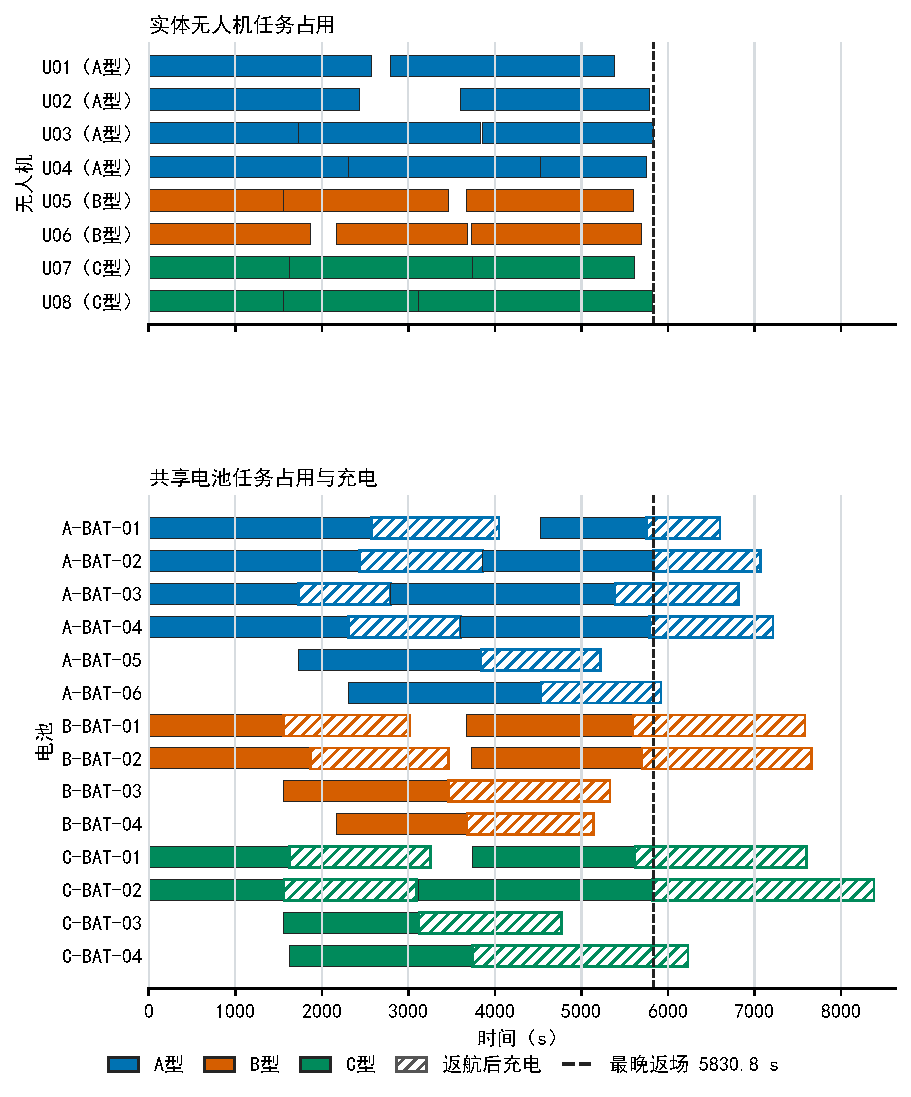
\includegraphics[height=0.82\textheight,keepaspectratio]{figures/q2_drone_battery_gantt.pdf}
\caption{问题二实体无人机与共享电池资源排程}
\label{fig:q2-gantt}
\end{figure}
\begin{figure}[htbp]
\centering
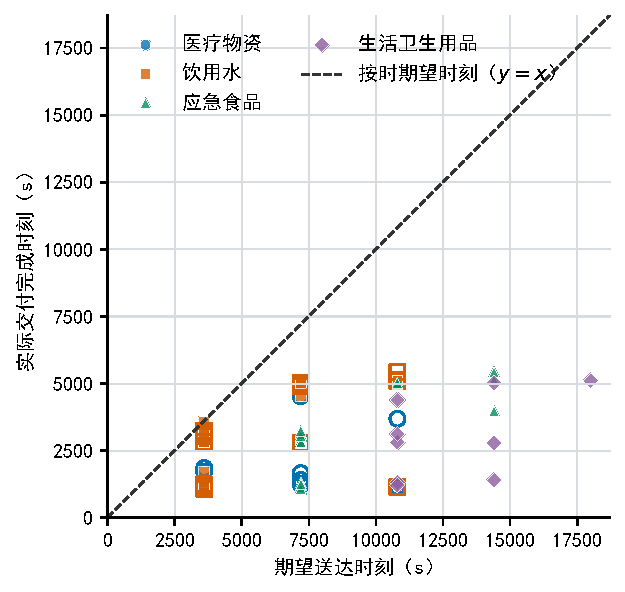
\includegraphics[width=0.82\textwidth]{figures/q2_expected_vs_actual_delivery.pdf}
\caption{货箱实际交付时刻与期望交付时刻对照}
\label{fig:q2-delivery}
\end{figure}
\clearpage
\subsection{独立可行性检验}

独立检查程序不读取求解器中间状态，而从导出的架次表和逐箱表重新构造所有航段。检查内容包括：80个货箱恰好出现一次；逐架次质量、体积、剩余载荷、能耗和返航SOC满足约束；逐箱交付时刻与路线递推一致；医疗及首批货箱全部满足硬时限；全部货箱不超过期望时刻；同一实体无人机任务区间无重叠；同一电池在上次返航并充至100\%后才可再次投入。新推荐方案通过全部检查；另外设置三个回归测试，核验等价类别定义、箱号还原与候选去重。该检验独立于调度算法，但沿用同一基础物理内核，不构成对能耗建模假设的独立实证验证。

\section{问题三：运输与中继无人机联合调度}

\subsection{连续通信判定模型}

问题三继承问题二的载荷、能量、时限及资源周转约束，并要求运输无人机在爬升、巡航、下降和物资交接全过程保持通信。本文将每个运输架次展开为分段连续三维轨迹；飞行段内经纬度和海拔按时间线性插值，交接段位置固定于服务区作业高度。

对任意通信端点 $i,j$，沿两点视线对DEM进行加密采样。若任一内部采样点地面高程不低于视线海拔，则令遮挡变量 $b_{ij}(t)=1$。传播损耗为
\[
L_{ij}(t)=32.45+20\log_{10}f+20\log_{10}D_{ij}(t)
            +L_{\rm obs}b_{ij}(t),
\]
其中 $f$ 以MHz计，$D$ 以km计。双向链路允许损耗取两个方向门限的较小值。由附件参数计算，运输机--G01直连、运输机--中继接入及中继--G01回传门限分别为122、116和126~dB。

若运输机与G01链路可用，则优先记为直连；否则仅当运输机--中继接入链路和中继--G01回传链路在同一时刻均可用时，记为中继状态。其余情况为通信中断，并作为不可行条件。

\subsection{候选悬停点与联合调度}

候选点必须位于DEM范围内、离地高度不超过300~m并满足回传链路可用。以既有三个中继点为起点，先在新运输航线上检验空间覆盖，再搜索邻域位置与高度。空间覆盖与时间可行性分开检查：即使三个点共同覆盖全部采样点，两架中继机也未必能在交付时限前完成返场、周转和再次建链。

本轮从问题二22架次、5830.82~s的方案出发。直接沿用原路线时，S009--S012和S007--S003航段出现旧驻守点未覆盖的短区间；仅调整驻守点得到的部分空间可行候选，又在资源与时限模型中不可行。最终只改变两个医疗箱的批次归属：将S002-MED-01由原Q2-003并入Q2-011，将S012-MED-01由Q2-004并入Q2-012，运输架次数仍为22。前者避免为了S002医疗箱提前执行S004任务，后者去掉S009--S012跨区航段；其余覆盖缺口通过西部中继位置调整消除。

对上述批次枚举物理可行机型和访问顺序，预计算中继需求相对区间，并在区间两端增加3~s时间缓冲。CP-SAT同时决定机型、顺序、开始时刻及三个中继窗口；运输无人机与电池分别设置容量约束，中继无人机占用区间延长至返场后300~s，从而允许两架中继机自由分配，而非固定数组中的任务归属。第一阶段最小化联合返场时刻，第二阶段保持该时间上界，最小化运输与中继总能耗；随后局部调整中继位置并再次排程。

最终为A型8架次、B型8架次、C型6架次。R02驻守西部点，R01先执行东南任务，再返场换组件执行北部任务。本方案的开始时刻、机型和部分访问顺序不同于Q2，不能把5830.82~s直接当作Q3结果。固定修正批次、位置和需求分配后的毫秒模型得到6926.152~s的最优值，但该结论不覆盖其他组批、驻守点或中继需求分配，不能宣称全局最优。

中继架次往返飞行时间沿用三阶段口径。水平能耗按巡航功率乘巡航时间计算，爬升附加能耗取计划起飞总质量；建链阶段计悬停功率，服务阶段计悬停功率与通信附加功率之和。各架次满足20\%返航余量，R02两架次之间另计300~s周转时间。

\subsection{联合调度结果}

\begin{table}[htbp]
\centering
\caption{问题三中继架次方案}
\small
\begin{tabular}{cllrrrrr}
\toprule
架次 & 中继机 & 组件 & 经度 & 纬度 & 海拔/m & 服务时段/s & 能耗/kWh\\
\midrule
R01 & R02 & EC01 & 109.2066528 & 23.0432443 & 744.723 & 2295.45--6414.61 & 1.5177\\
R02 & R01 & EC02 & 109.2663164 & 23.0128425 & 629.728 & 754.45--3331.71 & 0.9968\\
R03 & R01 & EC03 & 109.2312200 & 23.0612224 & 322.250 & 5894.82--6226.21 & 0.3770\\
\bottomrule
\end{tabular}
\end{table}

联合方案包含22个运输架次和3个中继架次，使用2架中继无人机及3组能源组件。80个货箱均按时交付，硬时限违约和普通物资迟到均为0。运输能耗为65.6721~kWh，中继能耗为2.8915~kWh，总能耗为68.5635~kWh。运输最晚返航与最后中继返场均约为6926.15~s，联合完成时间为6926.1512~s。

相对原24运输架次、6997.28~s、73.5972~kWh方案，新方案减少2个运输架次，联合完成时间缩短71.13~s（1.02\%），总能耗减少5.0337~kWh（6.84\%）。旧22架次、7970.9~s、70.4145~kWh方案也保留为历史对照，不再称为当前低能耗推荐。以上均为在统一口径下得到的可行结果，未证明3个中继架次或22个运输架次的全局最少性。

\subsection{独立检验与离散粒度}

独立程序从Q3输出重新构造80箱运输、无人机与电池时间线、中继往返飞行和能源组件时间线，并复算每个链路的地形遮挡、自由空间损耗和双向门限。0.5~s粒度复核66660个通信点，未发现中断。全部中继悬停点位于DEM范围内、离地高度不超过300~m，两架中继无人机无任务重叠，能源组件均满足返航余量和充满后复用要求。

进一步采用0.1~s时间粒度复核331961个通信点，未发现中断。该结论是离散采样验证，不能替代连续时间链路可用性的严格数学证明；时间缓冲也不等于链路功率的鲁棒裕度。下一章Q4已冻结本轮运输与中继关系，重新核算任务分区和独立资源需求。

\section{问题四：独立任务分区与资源配置}
\noindent{\heiti 版本说明：}本章已按最新Q3的22运输架次、3中继架次、6926.1512~s方案重算；运输与中继任务、通信保障关系均保持不变。

\subsection{任务继承与分区约束}

问题四严格继承问题三的货箱组批、访问顺序、起止时刻及通信保障关系，不再重排运输或中继任务。以15个服务区为顶点；若两个服务区出现在同一运输架次中，则将其强制合并，且合并关系具有传递性。新方案形成两个多站单元：\{S002,\allowbreak S009\}与\{S003,\allowbreak S007,\allowbreak S011,\allowbreak S015\}；其余9站各自独立，合计11个不可拆单元。

设服务区分组为$G_1,\ldots,G_K$，其中$K\in\{2,3\}$。各组非空、两两不交且并集为全部服务区。某组继承所有涉及该组服务区的运输架次；若某中继架次曾保障该组任一运输架次，则本模型为该组保留该中继的完整任务窗口。跨组共享同一中继时，在各组独立复制所需保障，不跨组调配资源。原题强制同组条款针对运输架次，并未要求同一中继保障的所有服务区合并；上述完整窗口复制是本章明确采用的保守核算假设，不等同于允许共享中继实体或截短原中继安排。

\subsection{峰值资源与分区目标}

对组$g$和机型$a$，运输无人机需求为任务区间的最大重叠数
\[
N^{\rm U}_{ga}=\max_t\sum_{r\in\mathcal R_{ga}}
\mathbf 1\{s_r\le t<e_r\}.
\]
共享电池从架次开始至返航后充满均视为占用，将$e_r$替换为充电完成时刻即可得到$N^{\rm B}_{ga}$。中继无人机占用至返航后300~s周转结束，能源组件占用至充满；两类中继资源同样按区间最大重叠数核算。时刻统一保留到0.001~s，避免输出舍入造成伪重叠。组内同型资源可以重新编号但不改变任务时刻，区间着色可实现峰值配置；因此资源需求不是Q3表中不同编号的机械计数。

组间工作量定义为该组全部运输与中继架次从开始至返航的时长之和，以变异系数
\[
CV=\frac{\sqrt{K^{-1}\sum_g(W_g-\bar W)^2}}{\bar W}
\]
衡量均衡性。沿用前轮建模选择，以$CV\le0.10$作为均衡目标，再依次最小化相对现有库存的资源总缺口、$CV$、货箱数极差、重复配置规模及空间离散度。10\%阈值不是题面硬约束；各类资源数量直接相加也不表示采购成本加总。对11个单元的$S(11,2)=1023$个两组分区和$S(11,3)=28501$个三组分区穷举，两者均有满足均衡目标的解。下述最优性仅针对冻结的Q3、完整中继窗口复制及给定目标次序成立。

\subsection{分区与资源配置结果}

\begin{table}[htbp]
\centering
\caption{两组任务分区及独立资源需求}
\small
\begin{tabular}{c p{5.2cm} *{8}{>{\centering\arraybackslash}p{0.8cm}}}
\toprule
组别 & 服务区 & \shortstack{A\\机} & \shortstack{B\\机} & \shortstack{C\\机} & \shortstack{A\\电池} & \shortstack{B\\电池} & \shortstack{C\\电池} & \shortstack{中继\\机} & 组件\\
\midrule
G1 & \shortstack[l]{S001,S003,S005,S006,\\S007,S011,S012,S015} & 3&1&2&4&1&3&2&2\\
G2 & \shortstack[l]{S002,S004,S008,S009,\\S010,S013,S014} & 2&2&1&3&3&1&2&2\\
\bottomrule
\end{tabular}
\end{table}

两组各承担11个运输架次；G1含49箱、2个中继任务副本，G2含31箱、3个中继任务副本。两组综合工作量分别为29844.080~s和31492.948~s，$CV=0.026882$。合计需A/B/C型运输机$5/3/3$架、对应电池$7/4/4$组、中继机4架和能源组件4组。

\begin{table}[htbp]
\centering
\caption{三组任务分区及独立资源需求}
\small
\begin{tabular}{c p{5.2cm} *{8}{>{\centering\arraybackslash}p{0.8cm}}}
\toprule
组别 & 服务区 & \shortstack{A\\机} & \shortstack{B\\机} & \shortstack{C\\机} & \shortstack{A\\电池} & \shortstack{B\\电池} & \shortstack{C\\电池} & \shortstack{中继\\机} & 组件\\
\midrule
G1 & \shortstack[l]{S001,S003,S005,\\S007,S011,S015} & 3&1&2&4&1&2&1&1\\
G2 & S002,S004,S009,S013 & 2&1&1&3&1&1&2&2\\
G3 & \shortstack[l]{S006,S008,S010,\\S012,S014} & 0&2&1&0&3&1&2&2\\
\bottomrule
\end{tabular}
\end{table}

三组分别承担9、7、6个运输架次，货箱数为40、20、20，中继任务副本数为1、3、2，综合工作量为22791.101、24197.998、19648.754~s，$CV=0.085615$。合计需A/B/C型运输机$5/4/4$架、对应电池$7/5/4$组、中继机5架和能源组件5组。

\subsection{两种方案比较与缺口原因}

\begin{table}[htbp]
\centering
\caption{两种分区方案的资源与均衡性比较}
\small
\begin{tabular}{crrrrrr}
\toprule
$K$ & 配置总数 & 重复配置数 & 库存缺口数 & 库存冗余数 & 工作量$CV$ & 货箱极差\\
\midrule
2 & 34 & 8 & 6 & 2 & 0.0269 & 18\\
3 & 39 & 13 & 10 & 1 & 0.0856 & 20\\
\bottomrule
\end{tabular}
\end{table}

现有库存为A/B/C型运输机$4/2/2$架、电池$6/4/4$组、中继机2架和能源组件6组。两组方案缺A/B/C型运输机各1架、A型电池1组和中继机2架，合计6个资源单位；三组方案缺A型机1架、B/C型机各2架、A/B型电池各1组和中继机3架，合计10个资源单位。两组与三组方案分别富余2组和1组中继能源组件，异类库存富余不能抵消其他类型的缺口。

不分区时，同一Q3任务的峰值需求为运输机$4/2/2$、电池$6/4/4$、中继机2架和组件2组，合计26个资源单位；虽然Q3方案使用了3个组件编号，按不变时间窗核算的峰值只需2组。分为两组和三组后分别重复配置8个和13个资源单位。

缺口主要来自跨组复用的丧失及中继保障的独立复制，而非运输任务增加。新Q3整体更省能、更快，并不保证分区后更省资源，因为多站批次和资源复用关系也发生了改变。本轮两组方案不仅配置规模和库存缺口较小，工作量$CV$及货箱极差也小于三组方案；三组提供更细的地域责任划分，但没有表现出更好的工作量均衡。因而在上述目标与核算口径下推荐两组方案；其执行仍以补齐所列缺口为前提。

\subsection{独立检验}

独立校验程序从Q3结果重新建立运输和中继占用区间，核对服务区互斥完备划分、多站批次不可拆、任务继承、资源峰值、逐项库存缺口及冗余、运输和中继能耗、综合工作量。两组与三组方案全部通过复核；另以三个回归测试检查同刻周转、充电重叠及同组约束的传递性。Q3输入快照及SHA-256清单随结果保存，确保上下游版本可追溯。官方结果表填入分区及资源数量，完整比较另存明细文件。


\begin{thebibliography}{2}
\bibitem{zhang2021}
J. Zhang, J. F. Campbell, D. C. Sweeney II, and A. C. Hupman,
``Energy consumption models for delivery drones: A comparison and assessment,''
\textit{Transportation Research Part D: Transport and Environment}, vol. 90,
art. 102668, 2021, doi: 10.1016/j.trd.2020.102668.

\bibitem{dorling2017}
K. Dorling, J. Heinrichs, G. G. Messier, and S. Magierowski,
``Vehicle routing problems for drone delivery,''
\textit{IEEE Transactions on Systems, Man, and Cybernetics: Systems}, vol. 47,
no. 1, pp. 70--85, Jan. 2017, doi: 10.1109/TSMC.2016.2582745.
\end{thebibliography}

\end{document}
